\documentclass[pageno]{jpaper}
%replace XXX with the submission number you are given from the ASPLOS submission site.
\newcommand{\asplossubmissionnumber}{XXX}

\usepackage[normalem]{ulem}
\begin{document}

\title{6.867 Machine Learning Homework 2 \& 3}
\date{}
\maketitle

\thispagestyle{empty}


\section{Support Vector Machine Classification}
In this section of we explore the use of support vector machines(SVM) for use in the task of classification. We will focus on implementing the SVM dual optimization problem. Additionally, we will implement the soft-margin SVM which contains a slack variable to allow for data points to be on the incorrect side of the decision boundary with some amount of tolerance. This soft margin allows us to classify points even in the situation when there is no linear separation between classes. This slack is parameterized by the variable C. As C increases the SVM approaches a hard-margin.The complete optimization problem that we seek to solve is shown below.
\begin{figure}[ht!]
\centering
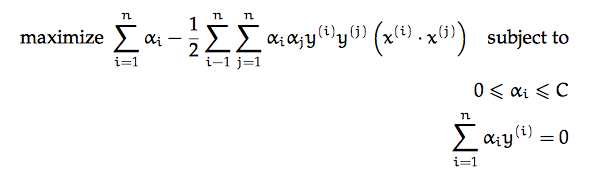
\includegraphics[width=70mm]{svm_dual_soft}
\end{figure}

We utilize the cvxopt quadratic programming toolbox for python in order to solve this convex optimization problem.
Once we optimize for the values of $\alpha$\ we must solve for $w_0$\ and $w$\, shown in the equations below. In the equation below M is the set of support vectors.

\begin{figure}[ht!]
\centering
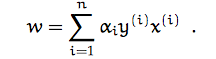
\includegraphics[width=30mm]{w}
\end{figure}

\begin{figure}[ht!]
\centering
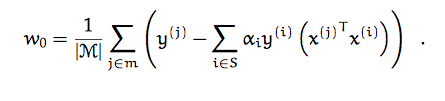
\includegraphics[width=60mm]{W_0}
\end{figure}

After computing $w_0$\ and $w$\ we have our decision boundary and apply the decision rule below to predict the label for subsequent data.

\begin{figure}[ht!]
\centering
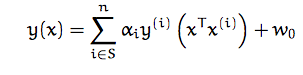
\includegraphics[width=40mm]{decision_rule}
\end{figure}

\subsection{}
In this section we test our implementation of the soft-margin SVM using the synthetic data with positive examples (1, 2), (2, 2) and negative examples (0, 0), (-2, 3). Table 1 shows the alphas resulting from solving the quadratic optimization problem, the Weight and W\_0 vectors as well as the accuracy of this classifier on the training set which is 100\%. Figure one shows the resulting decision boundary and classification of points. We can clearly see that our implementation is successful in producing the maximum margin separator for the training data.
\begin{table}[h!]
  \centering
  \begin{tabular}{llllll|}
    \hline
    \textbf{Alphas}  & \textbf{W}  & \textbf{W\_0} & \textbf{Accuracy}\\
    \hline
    \hline
 5.30612273e-01 	&0.85714299 &-1.21428584   &100\% \\
 \hline
3.11022745e-08	&0.57142862 	& & \\
 \hline
3.67346975e-01	& 	& & \\
 \hline
1.63265328e-01	& 	& & \\
 \hline
  \end{tabular}
  \caption{Optimal Alpha values, Weight vector, W\_0 vector and accuracy for basic dataset}
  \label{table:formatting}
\end{table}

\begin{figure}[ht!]
\centering
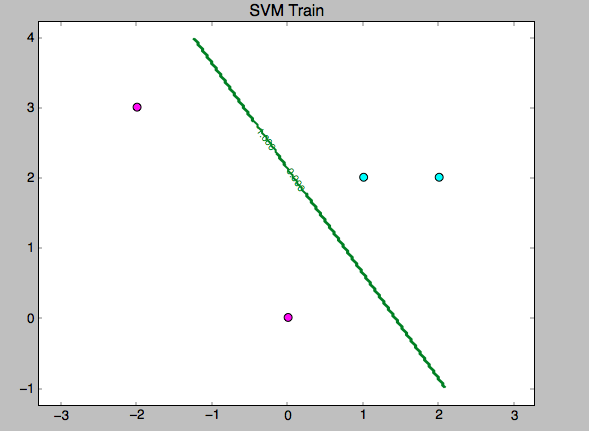
\includegraphics[width=60mm]{1_1_basic_synthetic}
\caption{SVM decision boundary using synthetic data points}
\label{overflow}
\end{figure}

Notice here that none of our $alpha$\ values are zero, yet the data should have produced only three support vectors not four. The model creates a support vector of the point furthest to the right, which it should not; this point should not affect the decision boundary. The value of alpha for this point is very low at 3.11022745e-08. We decided to threshold all alpha values at 1e-5; anything below this value is set to zero.

\subsection{}
In this section we test our classifier on the four given datasets, and observe the decision boundary and the classification error rate on the training and validation test sets. For all trials in this section hold the value of C equal to one. In all trails the training and the testing data contained 400 data points each. 
Figures 2 through 9 show the decision boundaries and the classes for each point in the training and testing set. Table 2 and 3 shows the number of support vectors, the values for W\_0 and W as well as the training and testing error for each dataset.

\begin{figure}[ht!]
\centering
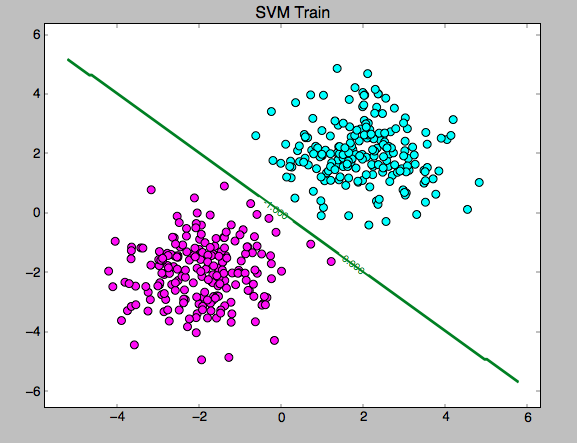
\includegraphics[width=60mm]{stdev1_train}
\caption{StDev1 Data Training}
\label{overflow}
\end{figure}

\begin{figure}[ht!]
\centering
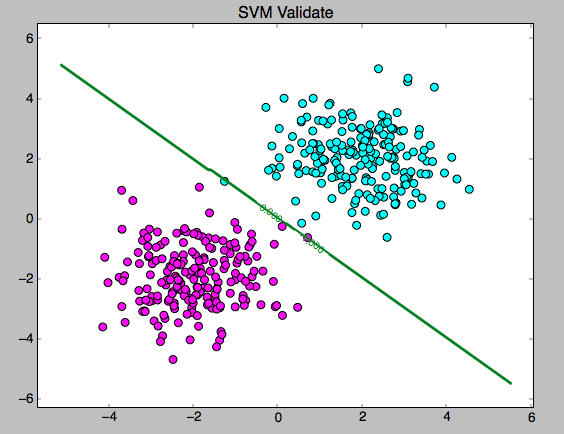
\includegraphics[width=60mm]{stdev1_test}
\caption{StDev1 Data Testing}
\label{overflow}
\end{figure}

\begin{figure}[ht!]
\centering
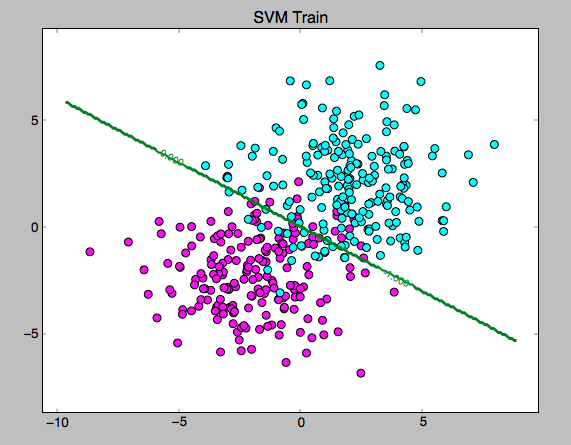
\includegraphics[width=60mm]{stdev2_train}
\caption{StDev2 Data Training}
\label{overflow}
\end{figure}

\begin{figure}[ht!]
\centering
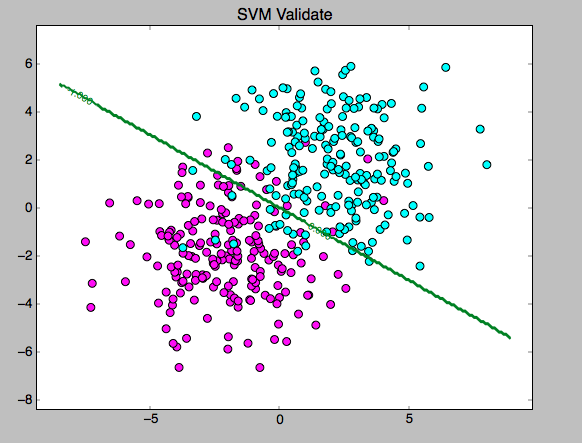
\includegraphics[width=60mm]{stdev2_test}
\caption{StDev2 Data Testing}
\label{overflow}
\end{figure}

\begin{figure}[ht!]
\centering
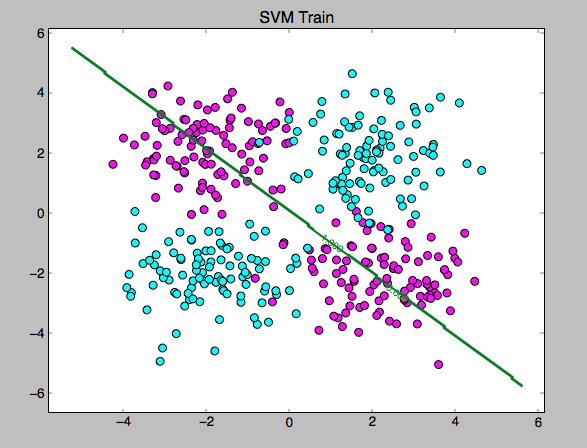
\includegraphics[width=60mm]{nonSep2_train}
\caption{NonSep2 Data Training}
\label{overflow}
\end{figure}

\begin{figure}[ht!]
\centering
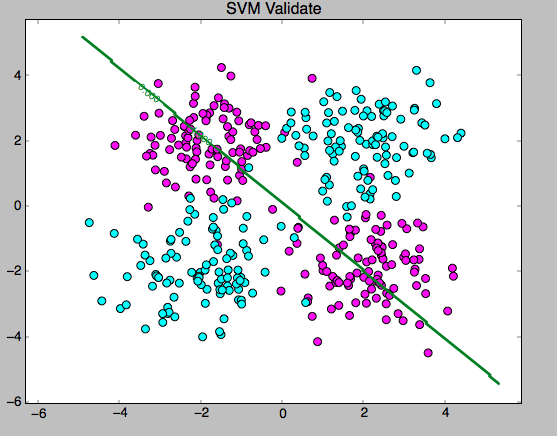
\includegraphics[width=60mm]{nonSep2_test}
\caption{NonSep2 Data Testing}
\label{overflow}
\end{figure}

\begin{figure}[ht!]
\centering
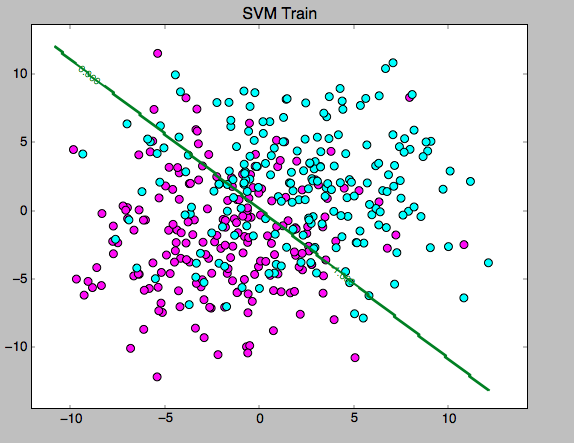
\includegraphics[width=60mm]{stdev4_train}
\caption{StDev4 Data Training}
\label{overflow}
\end{figure}

\begin{figure}[ht!]
\centering
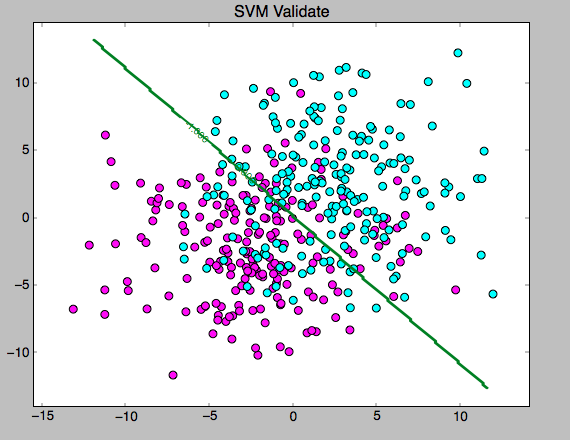
\includegraphics[width=60mm]{stdev4_test}
\caption{StDev4 Data Testing}
\label{overflow}
\end{figure}



\begin{table}[h!]
  \centering
  \begin{tabular}{llllll|}
    \hline
     \textbf{DataSet} &\textbf{\# S.V.}  & \textbf{W\_0}  & \textbf{W} \\
    \hline
    \hline
 \textbf{Stdev1} 	&5 &0.011 &1.233, 1.241  \\
 \hline
\textbf{Stdev2}	&91 	& 0.017 & 0.457, 0.755  \\
 \hline
\textbf{nonSep2}	&392 &0.005	 &-0.219, -0.211  \\
 \hline
\textbf{Stdev4}	&243 	&-0.006 &0.199, 0.182 \\
 \hline
 \end{tabular}
  \caption{Number of Support Vectors, Weight vector and W\_0 vector for various datasets}
  \label{table:formatting}
\end{table}

\begin{table}[h!]
  \centering
  \begin{tabular}{llllll|}
    \hline
     \textbf{DataSet}  & \textbf{Train Error} & \textbf{Test Error}\\
    \hline
    \hline
 \textbf{Stdev1} 	   &0.0\% & 0.5\%\\
 \hline
\textbf{Stdev2}	 & 9.5\% &8.0\% \\
 \hline
\textbf{nonSep2}	 &48.5\% &50.25\% \\
 \hline
\textbf{Stdev4}	 &26.5\% & 21.5\%\\
 \hline
 
  \end{tabular}
  \caption{Classification Error for various datasets}
  \label{table:formatting}
\end{table}

Visually if we observe the figures we can see that nonSep2 is not linearly separable and therefore achieves poor performance. As the data in sac class overlap more and more a linear decision boundary becomes more difficult to define. Stdev1, 2 and 4 are increasingly difficult to linearly separate and therefore achieve higher and higher errors.  Defining a separation boundary for any of these datasets other than Stdev1 is impossible with the hard margin SVM. Looking at table 2 and 3we see that as error increases so do the number of support vectors. This is due to the fact that as the data becomes more difficult to separate linearly, the number of support vectors increases so that more of the points define the decision boundary.

\subsection{}
In this section we extend our SVM dual implementation to operate with kernels. Table 4 shows the number of support vectors, and geometric margin for various values of C. We can see that as we increase C the number of support vectors decreases. This is due to the fact that as C increases we approach the hard margin SVM problem in which the boundary depends on less points. As C increases the value for the geometric margin decreases. This is due to the fact that as C increases we approach the hard margin SVM problem in which the margin is small. The value of C typically changes the resulting classifier and therefore affects the accuracy on the test samples. However, Maximizing the geometric margin on the training set would not be an appropriate criterion for selecting C, due to the fact that this will lead to overfitting. The resultant classifier would be very well tailored to the training set but would not generalize well to future unseen data. As an alternative we could find the optimal value of C on a validation set separate from the training set and then apply this model to a new testing set, alleviating the problem of overfitting. 
Table 5 shows the training and testing errors vs. C for two of the datasets. We can see that changing C does not have a drastic impact on the error for these two datasets.

\begin{table}[h!]
  \centering
  \begin{tabular}{llllll|}
    \hline
     \textbf{DataSet} &\textbf{\# C}  & \textbf{Number of alphas}  & \textbf{Geometric Margin} \\
    \hline
    \hline
 \textbf{Stdev1} 	&0.01 &52 &1.65  \\
 \hline
  \textbf{Stdev1} 	&0.1 &16 & 1.05  \\
 \hline
  \textbf{Stdev1} 	&1.0 &5 &0.57  \\
 \hline
  \textbf{Stdev1} 	&10 &3 &0.44  \\
 \hline
  \textbf{Stdev1} 	&100 &3 &0.44  \\
 \hline
  \textbf{Stdev4} 	&0.01 &249 & 3.89  \\
 \hline
  \textbf{Stdev4} 	&0.1 &243 &3.70  \\
 \hline
  \textbf{Stdev4} 	&1.0 &243 &3.70  \\
 \hline
  \textbf{Stdev4} 	&10 &256 &3.70  \\
 \hline
  \textbf{Stdev4} 	&100 &400 &3.70  \\
 \hline
 
 \end{tabular}
  \caption{Number of Alphas and Geometric Margin vs C values for datasets}
  \label{table:formatting}
\end{table}

\begin{table}[h!]
  \centering
  \begin{tabular}{llllll|}
    \hline
     \textbf{DataSet} &\textbf{\# C}  & \textbf{Train Error}  & \textbf{Test Error} \\
    \hline
    \hline
 \textbf{Stdev1} 	&0.01 &0.0\% & 0.0\%  \\
 \hline
  \textbf{Stdev1} 	&0.1 &0.00\% & 0.05\%  \\
 \hline
  \textbf{Stdev1} 	&1.0 &0.00\% &0.5\%  \\
 \hline
  \textbf{Stdev1} 	&10 &0.00\% &0.00\%  \\
 \hline
  \textbf{Stdev1} 	&100 &0.00\% &0.00\%  \\
 \hline
  \textbf{Stdev4} 	&0.01 &26.0\% & 21.75\%  \\
 \hline
  \textbf{Stdev4} 	&0.1 &26.50\% &21.50\%  \\
 \hline
  \textbf{Stdev4} 	&1.0 &26.50\% &21.50\%  \\
 \hline
  \textbf{Stdev4} 	&10 &26.0\% & 21.75\%  \\
 \hline
  \textbf{Stdev4} 	&100 &26.0\% & 21.75\%  \\
 \hline
 
 \end{tabular}
  \caption{Training and Testing Error vs. C values for datasets}
  \label{table:formatting}
\end{table}


\begin{table}[h!]
  \centering
  \begin{tabular}{llllll|}
    \hline
     \textbf{DataSet} &\textbf{\# 1/Bandwidth}  & \textbf{Train Error}  & \textbf{Test Error} \\
    \hline
    \hline

  \textbf{Stdev1} 	&0.25 &50.0\% & 50.0\%  \\
 \hline
  \textbf{Stdev1} 	&0.5 &0.00\% &2.25\%  \\
 \hline
  \textbf{Stdev1} 	&1.0 &0.00\% &0.25\%  \\
 \hline
   \textbf{Stdev1} 	&2.0 &0.00\% &0.25\%  \\
 \hline
  \textbf{Stdev2} 	&0.25 &50.0\% & 50.0\%  \\
 \hline
  \textbf{Stdev2} 	&0.5 &50.0\% &50.0\%  \\
 \hline
  \textbf{Stdev2} 	&1.0 &50.0\% &50.0\%  \\
 \hline
  \textbf{Stdev2} 	&2.0 &10.75\% &9.75\%  \\
   \hline
  \textbf{Stdev2} 	&2.0 &10.75\% &8.00\%  \\
  
 \hline
 \end{tabular}
  \caption{Training and Testing Error For Gaussian Kernel vs. 1/Bandwidth for datasets (C = 1)}
  \label{table:formatting}
\end{table}

Table 6 shows the training and testing error for two datasets as we vary the value 1/bandwidth. We can see that for dataset Stdev1 a value of 1.0 and for Stdev a value of 2 for 1/bandwidth provide excellent results. For all trials in table 6 the value of C was held constant to one. Figures 10 and 11 show the decision boundaries for training and testing for the Stdev1 dataset. We can see here that the RBF kernel is much more flexible than the linear kernel and in some cases may be able to provide for better classification.

\begin{figure}[ht!]
\centering
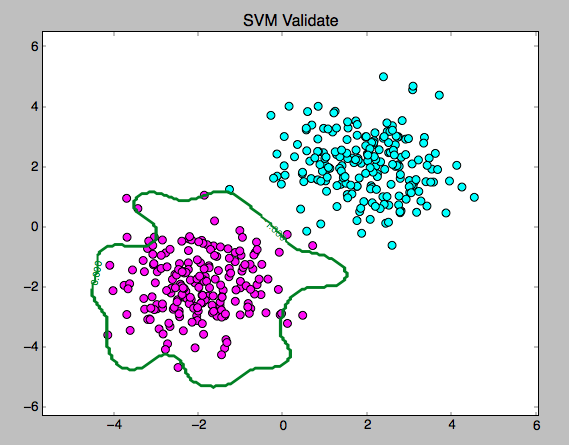
\includegraphics[width=60mm]{stdev1_gauss_train}
\caption{StDev1 RBF Training}
\label{overflow}
\end{figure}

\begin{figure}[ht!]
\centering
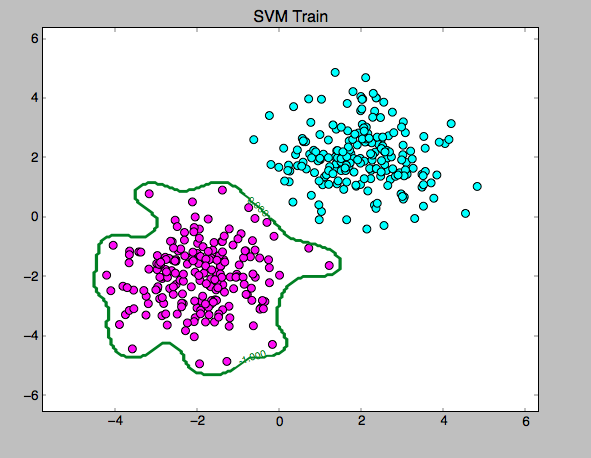
\includegraphics[width=60mm]{stdev1_gauss_test}
\caption{StDev1 RBF Kernel Testing}
\label{overflow}
\end{figure}


\section{Logistic Regression}

In this section we explore Logistic Regression for binary classification. Logistic regression is a discriminative model, where we are not making any distributional assumptions about X but rather only interested in the decision boundary. In logistic regression we look to minimize the following negative log likelihood shown in figure 12. Additionally we are interested in the kerneled version of logistic regression. To achieve this we simply substitute $W=X^{T}\alpha$\ .This allows us to represent the weight vector in terms of X and alphas. If we now look at the exponential term we see  $X^{i}X^{T}$\ which represents the kernelized form. To implement this optimization we utilized the scipy.optimize package, specifically the fmin\_bfgs function relating to the BFGS optimization algorithm. 

\begin{figure}[ht!]
\centering
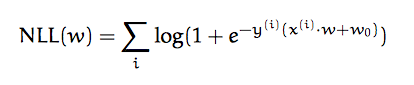
\includegraphics[width=70mm]{nll}
\caption{Logistic Regression Optimization}
\end{figure}
If the data is linearly separable then the optimization will want to make the weights as large as possible. To alleviate this we add a L1 regularization term around alpha. 

\begin{figure}[ht!]
\centering
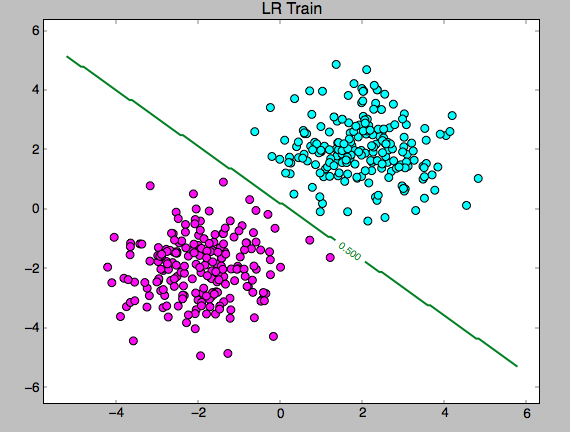
\includegraphics[width=60mm]{stdev1_lr_train}
\caption{StDev1 Logistic Regression Training}
\label{overflow}
\end{figure}
\subsection{}
\begin{figure}[ht!]
\centering
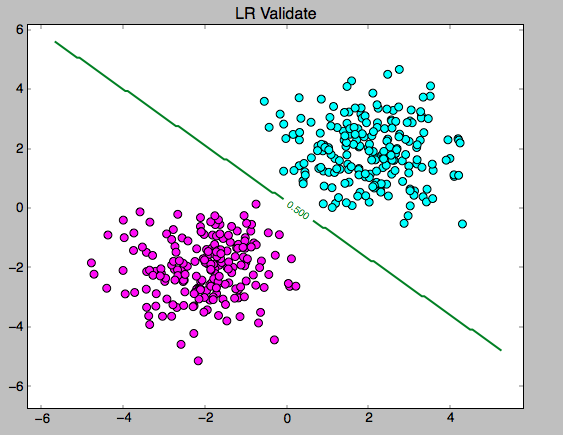
\includegraphics[width=60mm]{stdev1_lr_test}
\caption{StDev1 Logistic Regression Testing}
\label{overflow}
\end{figure}
\begin{figure}[ht!]
\centering
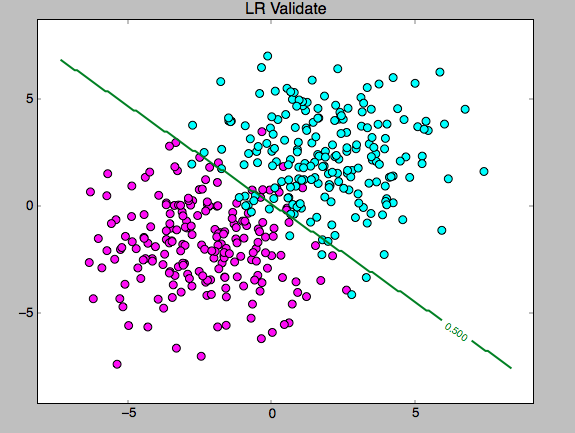
\includegraphics[width=60mm]{sdev2_lr_train}
\caption{StDev2 Logistic Regression Training}
\label{overflow}
\end{figure}
\subsection{}
\begin{figure}[ht!]
\centering
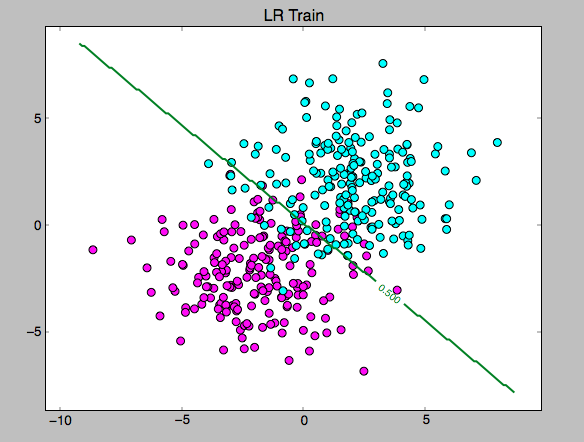
\includegraphics[width=60mm]{stdev2_lr_test}
\caption{StDev2 Logistic Regression Testing}
\label{overflow}
\end{figure}

\begin{table}[h!]
  \centering
  \begin{tabular}{llllll|}
    \hline
     \textbf{DataSet}  & \textbf{Number of Alphas} &\textbf{Train Error} & \textbf{Test Error}\\
    \hline
    \hline
 \textbf{Stdev1} 	   &400 &0.0\% & 0.0\%\\
 \hline
\textbf{Stdev2}	 &400 & 9.5\% &6.25\% \\
 \hline
\textbf{Stdev4}	 &400 &26.5\% & 24.0\%\\
 \hline
 
  \end{tabular}
  \caption{Classification Error for various datasets}
  \label{table:formatting}
\end{table}
\subsection{}
\begin{table}[h!]
  \centering
  \begin{tabular}{llllll|}
    \hline
     \textbf{DataSet} &\textbf{\# Lambda}  & & \textbf{Number of Alphas} \\
    \hline
    \hline

  \textbf{Stdev1} 	 & 0\%  &400\\
 \hline
  \textbf{Stdev1} 	 &0.0001\% &400  \\
 \hline
  \textbf{Stdev1} 	&0.001 &400  \\
 \hline
   \textbf{Stdev2} 	 & 0\%  &400\\
 \hline
  \textbf{Stdev2} 	 &0.0001\% &400  \\
 \hline
  \textbf{Stdev2} 	&0.001 &400  \\
 \hline
 \hline
 \end{tabular}
  \caption{Number of Alphas vs. Lambda}
  \label{table:formatting}
\end{table}

\subsection{}
\begin{table}[h!]
  \centering
  \begin{tabular}{llllll|}
    \hline
     \textbf{DataSet}  & \textbf{1/Bandwidth} &\textbf{Train Error} & \textbf{Test Error}\\
    \hline
    \hline
 \textbf{Stdev1} 	   &10 &1.75000\% & 0.75000\%\\
 \hline
  \textbf{Stdev1} 	   &5 &0.0\% & 0.0\%\\
 \hline
  \textbf{Stdev1} 	   &1 &0.0\% & 0.25000\%\\
 \hline
 \textbf{Stdev2} 	   &10 &50.00\% & 50.00\%\\
 \hline
  \textbf{Stdev2} 	   &5 &10.25000\% & 8.25000\%\\
 \hline
  \textbf{Stdev2} 	   &1 &50.00\% & 50.00\%\\
 \hline
  \end{tabular}
  \caption{1/Bandwidth vs. Train and Test Error for RBF Kernel}
  \label{table:formatting}
\end{table}
Table 9 shows the logistic regression with various bandwidths. A beta value of 2 achieves the best score on both datasets. Figure 17 and 18 show the RBF kernel with B=0.2 for the dataset stdv2. Similarly to the SVM the RBF kernel has more flexibly as compared to the linear kernel, so if tuned right can often achieve better performance. 
\begin{figure}[ht!]
\centering
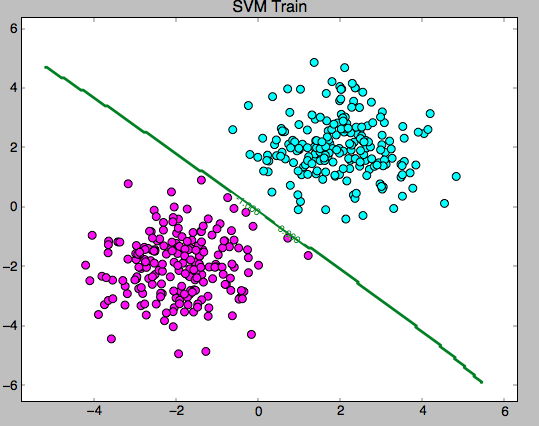
\includegraphics[width=60mm]{stdev1_rbf_lr_train_5}
\caption{StDev1 Logistic Regression RBF(B=.2)  Training}
\label{overflow}
\end{figure}
\begin{figure}[ht!]
\centering
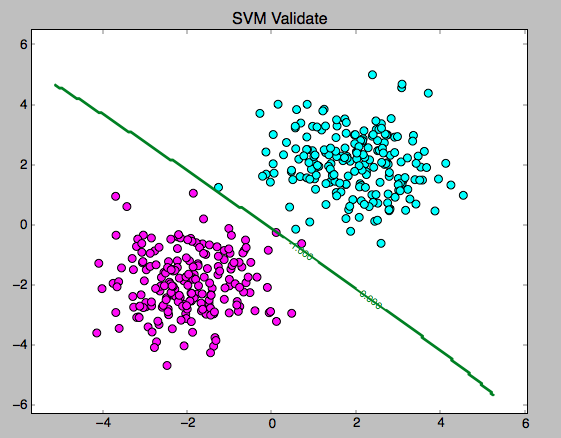
\includegraphics[width=60mm]{stdev1_rbf_lr_test_5}
\caption{StDev1 Logistic Regression RBF(B=.2) Testing}
\label{overflow}
\end{figure}
We can see that the SVM has much higher sparsity on alphas. The logistic regression model has a much higher number of alphas for the same dataset. This is due to the fact that the logistic regression model wants to increase the weights and therefore has more alphas greater than zero. Adding in a regularization term lessens the effect of large weights in the LR model but still does not reach the levels of sparsity as the SVM. The SVM model and the LR model do not select the same support vectors. Comparing at table 3 and at table 7 we can see that the SVM and the LR models preform almost equivalently well on the dataset. Due to the fact that LR is a discriminative model it does not converge on the non separable dataset. LR tries discriminate between the two classes and in that scenario it can not accomplish its objective and does not produce an output. A generative model such as Linear Discriminant Analysis will still provide a decision boundary even when the data are not linearly separable.

\section{Multi-Class Classification}
In the final section, we investigate multi-class classification for both SVM and logistic regression. SVMs are inherently binary classifiers. In order to expand them to be used in multiple class classification we must use a series of individual binary classifiers. There are a few approaches using this method, but we will focus on the one vs. rest approach. For this classifier we create K classifiers (where K is the number of classes) and classify each point as belonging to one class or belonging to the remainder of classes, and repeat this for all K-classes. Then for each point we take the class that gives it the highest score and classify it as belonging to that class. Although this classifier has its faults, such as uneven distributions when comparing one class to the remainder of the classes, it is efficient for large data sets.\\
Unlike SVMs, logistic regression is more easily extended to a multi-class classifier. Figure 15 shows the optimization objective for multi-class logistic regression. Unlike SVMs we can change the objective to extend to multi class rather than using multiple classifiers.\\
\begin{figure}[ht!]
\centering
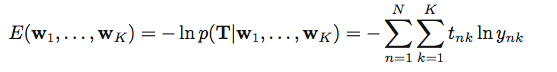
\includegraphics[width=70mm]{nll_mc}
\caption{Logistic Regression Multiclass Optimization}
\end{figure}
We test our implementations of the multi-class versions of SVMs and Logistic Regression on the Kaggle Dataset provided. Due to the extremely large size of the Kaggle dataset and the fact that our code has not been optimized for efficiency, we use a subset of the Kaggle Dataset to test on. We use 800 randomly selected data points for training and another 800 for testing. The Kaggle dataset contains 54 feature X values and 7 classes. 

\begin{table}[h!]
  \centering
  \begin{tabular}{llllll|}
    \hline
     \textbf{was } &\textbf{Error Train 1} & \textbf{Error Test 1} &\textbf{Error Train 2 }  & \textbf{Error Test 2}\\
    \hline
    \hline

  \textbf{SVM Linear} 	 & 19\%  &53.5\% &45.75\% &66.25\% &\\
 \hline
  \textbf{SVM RBF(B=.2)} 	 &54.25\% &77.75\% &38\% &38\%  \\
 \hline

   \textbf{SVM RBF(B=1)} 	&54.25\% &77.75\% & &   \\
 \hline
    \textbf{SVM RBF(B=.1)} 	&82.00\% &82.50\%  & &   \\
 \hline
 
   \textbf{LR Linear} 	 &34\% &55.2\% &54\%  & 54\% \\
 \hline
  \textbf{LR RBF(B=.2)} 	 &68\% &51.25\% \%  \\
 \hline


 \end{tabular}
  \caption{Errors for various SVM and LR on Kaggle Dataset}
  \label{table:formatting}
\end{table}
Note: due to the long runtimes, occasionally tests on data set 2 were excluded to allow for more implementations to be tried. 
Overall I found that the SVM multi-class outperformed the multi-class Logistic Regression. Due to the fact that only 800 points were used for training and testing each in each set, this does not give any conclusive evidence of the entire dataset. Additionally the 800 points contained all 7 classes thus allowing for a small amount of data comparatively about each class. Specifically the linear SVM outperformed the rest, while in general the error rates were relatively high. For future work, it would be interesting to use the sklearn implementations and try a variety of kernels and parameters for the entire dataset.

\end{document}

